% ---------------------------------------------------------------------------
% Variante USPSC 3.2 da monografia — exigência institucional (CHECKLIST §0.2).
%
% A classe USPSC é derivada de abntex2.cls v1.9.5 e é mantida pela Biblioteca
% do Campus USP de São Carlos. O corpo do texto NÃO é duplicado aqui: este
% arquivo carrega `uspsc/_body.tex`, extraído de `paper.tex` sem alteração, de
% modo que só existe uma fonte canônica de conteúdo.
%
% Compilar de dentro de docs/thesis (duas passagens):
%   pdflatex -interaction=nonstopmode paper-uspsc.tex
%   pdflatex -interaction=nonstopmode paper-uspsc.tex
%
% Regenerar o corpo após editar paper.tex:
%   python scripts/sync-uspsc-body.py
% ---------------------------------------------------------------------------
\documentclass[
12pt,
openright,
twoside,
a4paper,
chapter=TITLE,
english,
brazil
]{uspsc/USPSC-classe/USPSC}

\usepackage[utf8]{inputenc}
\usepackage[T1]{fontenc}
\usepackage{lmodern}
\usepackage{microtype}
\usepackage{amsmath}
\usepackage{booktabs}
\usepackage{multirow}
\usepackage{tabularx}
\usepackage{array}
\usepackage{graphicx}
% A folha de rosto da classe USPSC usa \nohyphens; sem hyphenat a compilação
% acusa "Undefined control sequence" ao montar os pré-textuais.
\usepackage{hyphenat}
\usepackage{pdfpages}   % \includepdf, usado pela ficha catalográfica oficial
\usepackage{tikz}
\usetikzlibrary{arrows.meta,positioning,shapes.geometric,fit,calc}
\usepackage{pgfplots}
\pgfplotsset{compat=1.18}

% NOTA — `USPSC-classe/ABNT6023-10520.sty` NÃO é carregado aqui.
% Esse arquivo pressupõe `abntex2cite` (sistema BibTeX) já carregado: ele chama
% \addtociteoptionlist, definido por aquele pacote. Este documento usa
% `thebibliography` manual, então carregá-lo aborta a compilação com
% "Undefined control sequence". A migração para .bib + abntex2cite é o passo
% seguinte da conformidade (CHECKLIST §5); enquanto ela não ocorre, as entradas
% seguem formatadas manualmente conforme a NBR 6023.
\usepackage{hyperref}
\hypersetup{colorlinks=true,linkcolor=black,citecolor=black,urlcolor=black}
\DeclareUrlCommand\codigo{\urlstyle{tt}}
\newcommand{\micro}{\,$\mu$s}
\newcommand{\svnota}[1]{\begin{center}\fbox{\begin{minipage}{0.90\textwidth}\textbf{#1}\end{minipage}}\end{center}}

% ---------------------------------------------------------------------------
% Identificação institucional. `MBAIAp` é a sigla oficial do programa para o
% MBA em Inteligência Artificial e Big Data em português; ela define
% \tipotrabalho, \area e o \preambulo padronizados pela Unidade, definidos em
% uspsc/USPSC-pre-textual-ICMC.tex — por isso esses campos NÃO são
% redefinidos aqui.
% ---------------------------------------------------------------------------
% `ICMC` (não `ICMC-TCC`) é a sigla que a classe roteia para
% USPSC-pre-textual-ICMC.tex, único arquivo do pacote que define o programa
% MBAIAp — a monografia de MBA usa o modelo de teses/dissertações da Unidade,
% não o de TCC de graduação (que só conhece BCCp/BSIp).
\siglaunidade{ICMC}
\programa{MBAIAp}

\titulo{Arquitetura de Soberania de Dados para Agentes de IA Pessoais: Um Modelo Local-First Baseado em Protocolos Descentralizados}
\autor{Pedro Henrique Almeida Prado de Oliveira}
\local{São Carlos}
\data{2026}
\orientador{Profa. Dra. Kalinka Regina Lucas Jaquie Castelo Branco}

\begin{document}
\pretextual
\imprimircapa

% A variante com estrela termina em \newpage, deixando o conteúdo seguinte no
% verso da folha de rosto — onde a NBR 14724 exige a ficha catalográfica.
\imprimirfolhaderosto*

% ---------------------------------------------------------------------------
% Ficha catalográfica — gerar na Biblioteca Achille Bassi (ICMC/USP) e salvar
% o PDF devolvido como uspsc/fichacatalografica.pdf. Com o arquivo presente,
% trocar o bloco de aviso abaixo por:
%   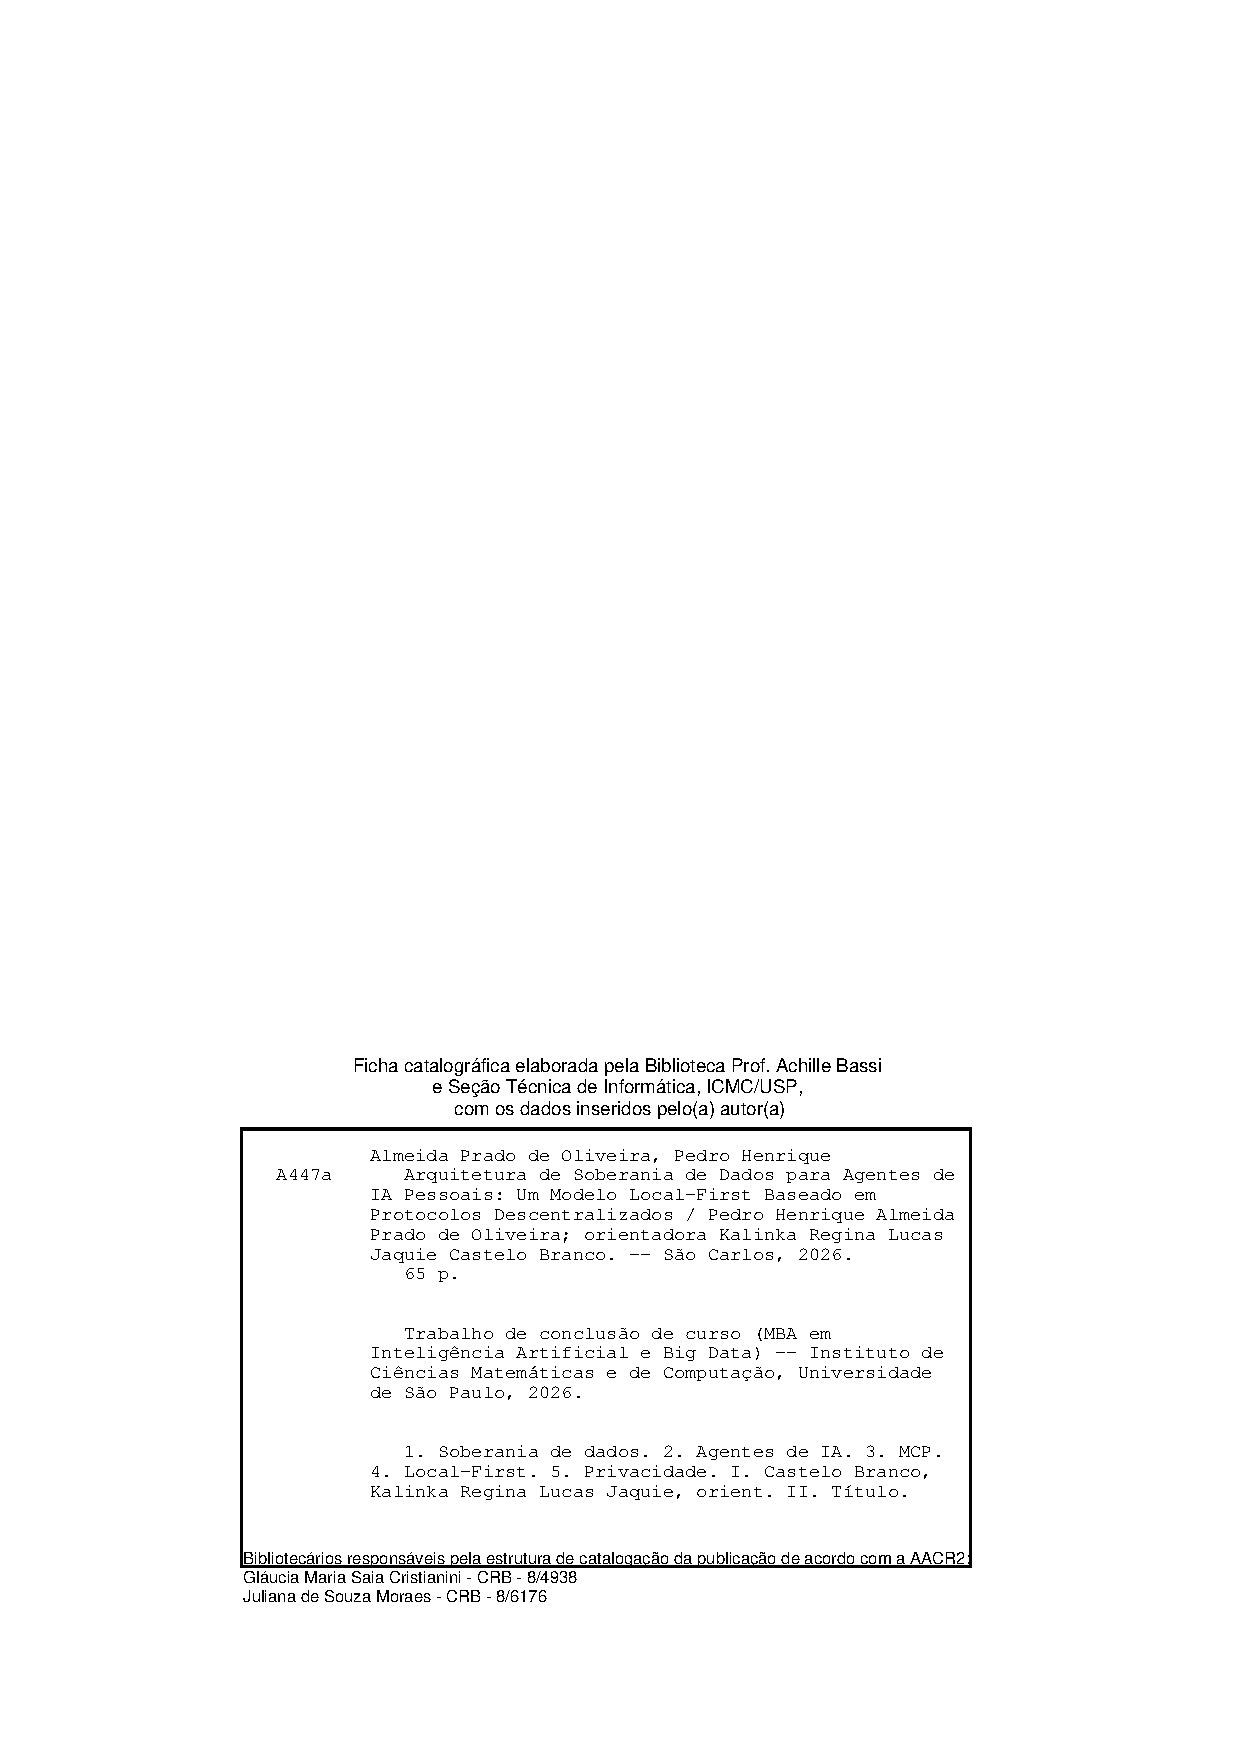
\includepdf{uspsc/fichacatalografica.pdf}
% ---------------------------------------------------------------------------
\begin{fichacatalografica}
\vspace*{\fill}
\begin{center}
\fbox{\begin{minipage}{12.5cm}
\vspace{0.3cm}
\textbf{[FICHA CATALOGRÁFICA A GERAR]}\par
Elemento obrigatório (NBR 14724). Gerar no sistema da Biblioteca Achille Bassi
(ICMC/USP) e substituir este bloco pelo PDF devolvido, sem reformatação.
\vspace{0.3cm}
\end{minipage}}
\end{center}
\end{fichacatalografica}

\begin{folhadeaprovacao}
\begin{center}
{\ABNTEXchapterfont\large\imprimirautor}

\vspace*{\fill}\vspace*{1.2cm}
\begin{minipage}[t]{\textwidth}
\centering
\ABNTEXchapterfont\bfseries\large\imprimirtitulo
\end{minipage}
\vspace*{1.2cm}

\hspace{.45\textwidth}
\begin{minipage}{.5\textwidth}
\imprimirpreambulo
\end{minipage}
\vspace*{1.2cm}

\end{center}

Trabalho aprovado. São Carlos, \rule[-0.2cm]{2.5cm}{0.15mm} de
\rule[-0.2cm]{4cm}{0.15mm} de \rule[-0.2cm]{1.5cm}{0.15mm}.

\vspace{1.0cm}
\begin{center}
\rule{9cm}{0.15mm}\par
\imprimirorientador\ (Orientador(a))

\vspace{1.0cm}
\rule{9cm}{0.15mm}\par
{}[MEMBRO DA BANCA 1]

\vspace{1.0cm}
\rule{9cm}{0.15mm}\par
{}[MEMBRO DA BANCA 2]
\end{center}
\vspace*{\fill}
\end{folhadeaprovacao}

% GERADO AUTOMATICAMENTE por scripts/sync-uspsc-body.py — NÃO EDITAR.
% Fonte canônica: docs/thesis/paper.tex


\begin{resumo}
Esta pesquisa implementa uma arquitetura \textit{Local-First} para mediar acessos de agentes de IA a segredos e credenciais locais. A instância avaliada, denominada \textit{Sovereign Vault}, combina cofre cifrado, \textit{gateway} MCP (\textit{Model Context Protocol}), escopos de capacidade, modos de consentimento e auditoria com evidência de adulteração. Sob protocolo corrigido de medição ($k=10$ sessões, ordem de células aleatorizada, mediana com intervalo de confiança de 95\% por \textit{bootstrap}), o custo do \textit{gate} de consentimento sob \textit{AutoAllow} é indistinguível de zero nos seis contrastes pareados; a imposição de escopos no caminho \textit{WebSocket} apresenta diferenças entre 2,1 e 2,2~$\mu$s com 20 escopos, sob ordem fixa dos braços, sem separar o efeito de escopo do efeito de posição; e a extensão da bateria adversarial pré-especificada elevou a cobertura da superfície de 20 ferramentas MCP de 5/20 para 17/20, revelando um defeito real de imposição de escopos no modo \textit{headless}. A avaliação atual é deliberadamente limitada a um \textit{microbenchmark} local sintético e a uma bateria finita de chamadas de ferramenta; não mede inferência em nuvem, utilidade de tarefa, tempo de decisão humana ou o custo da escrita de auditoria, excluído da soma de estágios instrumentada. No modo \textit{ANONYMIZED}, nomes completos, endereços, RG, CEP e telefones sem formatação passam sem máscara: mesmo com CPF ou CNPJ mascarados, um documento com nome e endereço pode permanecer identificável sob o Art.~5º da LGPD. Assim, o artefato não é adequado a documentos em que a vinculação de identidade por campos não mascarados seja risco realista.\par
\textbf{Palavras-chave}: soberania de dados; agentes de IA; MCP; Local-First; privacidade.
\end{resumo}
\begin{resumo}[Abstract]
\begin{otherlanguage*}{english}
This research proposes a Local-First architecture to mediate AI-agent access to local secrets and credentials. The evaluated instance, called Sovereign Vault, combines an encrypted vault, an MCP gateway, capability scopes, consent modes, and auditability with tamper evidence. Under a corrected measurement protocol ($k=10$ sessions, randomized cell order, median with 95\% bootstrap confidence intervals), the cost of the consent gate under AutoAllow is indistinguishable from zero in all six paired contrasts; scope measurements on the WebSocket path show differences between 2.1 and 2.2~$\mu$s with 20 scopes under fixed arm order, with scope count and execution position not separated; and the extension of the pre-specified adversarial battery raised coverage of the 20-tool MCP surface from 5/20 to 17/20, revealing a real scope-enforcement defect in headless mode. The current evaluation is deliberately limited to a synthetic local microbenchmark and a finite suite of tool calls; it does not measure cloud inference, task utility, human decision time, or the cost of the audit write, which is excluded from the instrumented stage sum. In ANONYMIZED mode, full names, addresses, Brazilian RG identification numbers, CEP postal codes, and unformatted telephone numbers pass through unmasked: even with Brazilian CPF or CNPJ identifiers masked, a document containing a name and address may remain identifiable under Article 5 of the LGPD. Therefore, the artifact is not suitable for documents in which identity linkage through unmasked fields is a realistic risk.
\end{otherlanguage*}
\textbf{Keywords}: data sovereignty; AI agents; MCP; Local-First; privacy.
\end{resumo}
\pdfbookmark[0]{\listfigurename}{lof}
\listoffigures*
\cleardoublepage
\pdfbookmark[0]{\listtablename}{lot}
\listoftables*
\cleardoublepage
\begin{siglas}
\item[IA] Inteligência Artificial
\item[LLM] Large Language Model
\item[MCP] Model Context Protocol
\item[DSR] Design Science Research
\item[SaaS] Software as a Service
\item[RAG] Retrieval-Augmented Generation
\item[LGPD] Lei Geral de Proteção de Dados
\item[GDPR] General Data Protection Regulation
\item[PII] Personally Identifiable Information
\item[RFC] Request for Comments
\item[ADR] Architecture Decision Record
\item[FEDS] Framework for Evaluation in Design Science Research
\item[HITL] Human-in-the-Loop
\item[KEK] Key Encryption Key
\item[DEK] Data Encryption Key
\item[OTP] One-Time Password
\item[CSP] Content Security Policy
\item[HMAC] Hash-based Message Authentication Code
\item[JSON-RPC] JavaScript Object Notation Remote Procedure Call
\item[WAN] Wide Area Network
\item[IC] Intervalo de Confiança
\end{siglas}
\tableofcontents*


\input{uspsc/_body}

\end{document}
